\documentclass[10pt,a4paper,titlepage,oneside]{memoir}

%% Packages
%% ========


\usepackage[OT1]{fontenc}
\usepackage[english]{babel}
\usepackage[utf8]{inputenc}
\usepackage[sc]{mathpazo}
\usepackage{amsmath,amssymb,amsfonts,mathrsfs}
\usepackage[amsmath,thmmarks]{ntheorem}
\usepackage{cite}
\usepackage{natbib}

%% LaTeX' own graphics handling
\usepackage{graphicx}
\graphicspath{{./images/}}
\DeclareGraphicsExtensions{.pdf,.png,.jpg,.eps,.tif}
\usepackage{epspdfconversion}
\usepackage{float}
\usepackage{wrapfig}
\usepackage{subfig}
\usepackage{soul}

%% See the TeXed file for more explanations

%% [OPT] Multi-rowed cells in tabulars
%\usepackage{multirow}

%% [REC] Intelligent cross reference package. This allows for nice
%% combined references that include the reference and a hint to where
%% to look for it.
\usepackage{varioref}

%% [OPT] Easily changeable quotes with \enquote{Text}
%\usepackage[german=swiss]{csquotes}

%% [REC] Format dates and time depending on locale
\usepackage{datetime}

%% [OPT] Provides a \cancel{} command to stroke through mathematics.
%\usepackage{cancel}

%% [NEED] This allows for additional typesetting tools in mathmode.
%% See its excellent documentation.
\usepackage{mathtools}

%% [ADV] Conditional commands
%\usepackage{ifthen}

%% [OPT] Manual large braces or other delimiters.
%\usepackage{bigdelim, bigstrut}

%% [REC] Alternate vector arrows. Use the command \vv{} to get scaled
%% vector arrows.
\usepackage[h]{esvect}

%% [NEED] Some extensions to tabulars and array environments.
\usepackage{array}

%% [OPT] Postscript support via pstricks graphics package. Very
%% diverse applications.
%\usepackage{pstricks,pst-all}

%% [?] This seems to allow us to define some additional counters.
%\usepackage{etex}

%% [ADV] XY-Pic to typeset some matrix-style graphics
%\usepackage[all]{xy}

%% [OPT] This is needed to generate an index at the end of the
%% document.
%\usepackage{makeidx}



%% [OPT] Fancy package for source code listings.  The template text
%% needs it for some LaTeX snippets; remove/adapt the \lstset when you
%% remove the template content.
\usepackage{listings}
\lstset{basicstyle=\scriptsize\ttfamily, 
		columns=fullflexible,
		keywordstyle=\color{red}\bfseries, 
		commentstyle=\color{OliveGreen},
		language=Matlab, 
		numbers=left, 
		numberstyle=\tiny, 
		stepnumber=1, 
		numbersep=5pt,
		frame=single, 
		captionpos=b, 
		breaklines=true, 
		breakatwhitespace=false,
		title=\lstname, 
		columns=fullflexible}

%% [REC] Fancy character protrusion.  Must be loaded after all fonts.
\usepackage[activate]{pdfcprot}

%% [REC] Nicer tables.  Read the excellent documentation.
\usepackage{booktabs}

%% Memoir layout setup

% Dependencies
\usepackage{ETHlogo}

% Turn extra space before chapter headings off.
\setlength{\beforechapskip}{0pt}

\nonzeroparskip
\parindent=0pt
\defaultlists

% Chapter style redefinition
\makeatletter

\if@twoside
  \pagestyle{Ruled}
  \copypagestyle{chapter}{Ruled}
\else
  \pagestyle{ruled}
  \copypagestyle{chapter}{ruled}
\fi
\makeoddhead{chapter}{}{}{}
\makeevenhead{chapter}{}{}{}
\makeheadrule{chapter}{\textwidth}{0pt}
\copypagestyle{abstract}{empty}

\makechapterstyle{bianchimod}{%
  \chapterstyle{default}
  \renewcommand*{\chapnamefont}{\normalfont\Large\sffamily}
  \renewcommand*{\chapnumfont}{\normalfont\Large\sffamily}
  \renewcommand*{\printchaptername}{%
    \chapnamefont\centering\@chapapp}
  \renewcommand*{\printchapternum}{\chapnumfont {\thechapter}}
  \renewcommand*{\chaptitlefont}{\normalfont\huge\sffamily}
  \renewcommand*{\printchaptertitle}[1]{%
    \hrule\vskip\onelineskip \centering \chaptitlefont\textbf{\vphantom{gyM}##1}\par}
  \renewcommand*{\afterchaptertitle}{\vskip\onelineskip \hrule\vskip
    \afterchapskip}
  \renewcommand*{\printchapternonum}{%
    \vphantom{\chapnumfont {9}}\afterchapternum}}

% Use the newly defined style
\chapterstyle{bianchimod}

\setsecheadstyle{\Large\bfseries\sffamily}
\setsubsecheadstyle{\large\bfseries\sffamily}
\setsubsubsecheadstyle{\bfseries\sffamily}
\setparaheadstyle{\normalsize\bfseries\sffamily}
\setsubparaheadstyle{\normalsize\itshape\sffamily}
\setsubparaindent{0pt}

% Set captions to a more separated style for clearness
\captionnamefont{\sffamily\bfseries\footnotesize}
\captiontitlefont{\sffamily\footnotesize}
\setlength{\intextsep}{16pt}
\setlength{\belowcaptionskip}{1pt}

% Set section and TOC numbering depth to subsection
\setsecnumdepth{subsection}
\settocdepth{subsection}

%% Titlepage adjustments

\pretitle{\vspace{25pt}\begin{center}\Large\sffamily\@thesistype\\\bfseries\HUGE}
\posttitle{\end{center}\par}
\preauthor{\vspace{0.5in}\par\begin{center}\let\and\\\Large\sffamily}
\postauthor{\end{center}}
\predate{\par\begin{center}\Large\sffamily}
\postdate{\end{center}\vspace{20pt}}

\def\@advisors{}
\newcommand{\advisors}[1]{\def\@advisors{#1}}
\def\@department{}
\newcommand{\department}[1]{\def\@department{#1}}
\def\@thesistype{}
\newcommand{\thesistype}[1]{\def\@thesistype{#1}}

\renewcommand{\maketitlehooka}{\vspace{-30pt}
\noindent\ETHlogo[2.5in]
\begin{flushright}
    \sffamily
    \@advisors\par
    \@department \\ ETH Z\"urich			
  \end{flushright}
  }

\settypeblocksize{8.5in}{6in}{*}
%Memoir: Set L & R margins around the type block:
%\setlrmargins{0cm}{0cm}{*}
%\settrims{0pt}{0pt}

\setlrmargins{*}{*}{*} %equal L & R margins ( = 2.5cm)

\checkandfixthelayout

\setlength{\droptitle}{-80pt}

\makeatother

% This defines how theorems should look. Best leave as is.
\theoremstyle{plain}
\setlength\theorempostskipamount{0pt}


%% Theorem-like environments

%% This can be changed according to language. You can comment out the ones you
%% don't need.

\numberwithin{equation}{chapter}

%% German theorems
%\newtheorem{satz}{Satz}[chapter]
%\newtheorem{beispiel}[satz]{Beispiel}
%\newtheorem{bemerkung}[satz]{Bemerkung}
%\newtheorem{korrolar}[satz]{Korrolar}
%\newtheorem{definition}[satz]{Definition}
%\newtheorem{lemma}[satz]{Lemma}
%\newtheorem{proposition}[satz]{Proposition}

%% English variants
\newtheorem{theorem}{Theorem}[chapter]
\newtheorem{example}[theorem]{Example}
\newtheorem{remark}[theorem]{Remark}
\newtheorem{corollary}[theorem]{Corollary}
\newtheorem{definition}[theorem]{Definition}
\newtheorem{lemma}[theorem]{Lemma}
\newtheorem{proposition}[theorem]{Proposition}

%% Proof environment with a small square as a "qed" symbol
\theoremstyle{nonumberplain}
\theorembodyfont{\normalfont}
\theoremsymbol{\ensuremath{\square}}
\newtheorem{proof}{Proof}
%\newtheorem{beweis}{Beweis}

%% Custom commands
%% ===============

%% Special characters for number sets, e.g. real or complex numbers.
\newcommand{\C}{\mathbb{C}}
\newcommand{\K}{\mathbb{K}}
\newcommand{\N}{\mathbb{N}}
\newcommand{\Q}{\mathbb{Q}}
\newcommand{\R}{\mathbb{R}}
\newcommand{\Z}{\mathbb{Z}}
\newcommand{\X}{\mathbb{X}}

%% Fixed/scaling delimiter examples (see mathtools documentation)
\DeclarePairedDelimiter\abs{\lvert}{\rvert}
\DeclarePairedDelimiter\norm{\lVert}{\rVert}

%% Use the alternative epsilon per default and define the old one as \oldepsilon
\let\oldepsilon\epsilon
\renewcommand{\epsilon}{\ensuremath\varepsilon}

%% Also set the alternate phi as default.
\let\oldphi\phi
\renewcommand{\phi}{\ensuremath{\varphi}}


\usepackage[linkcolor=black,colorlinks=true,citecolor=black,filecolor=black]{hyperref}


%% Document information
%% ====================

\title{Assignment \#01}
\author{Stephanie Fingerhuth, Lorenzo Gatti}
\thesistype{Synthetic Biology}
\department{Department of Computer Science}
\date{\today}

\begin{document}

%% Title page is autogenerated from document information above.  DO
%% NOT CHANGE.

\calccentering{\unitlength}
\begin{adjustwidth*}{\unitlength-45pt}{-\unitlength-45pt}
	\maketitle
\end{adjustwidth*}

%% TOC with the proper setup, do not change.
%\cleartorecto
%\tableofcontents

\renewcommand{\thefootnote}{\fnsymbol{footnote}}
\newcommand{\package}{\emph}

\setcounter{chapter}{1}
\setcounter{section}{0}

\section{a}

\begin{figure}[h!]
 \centering
    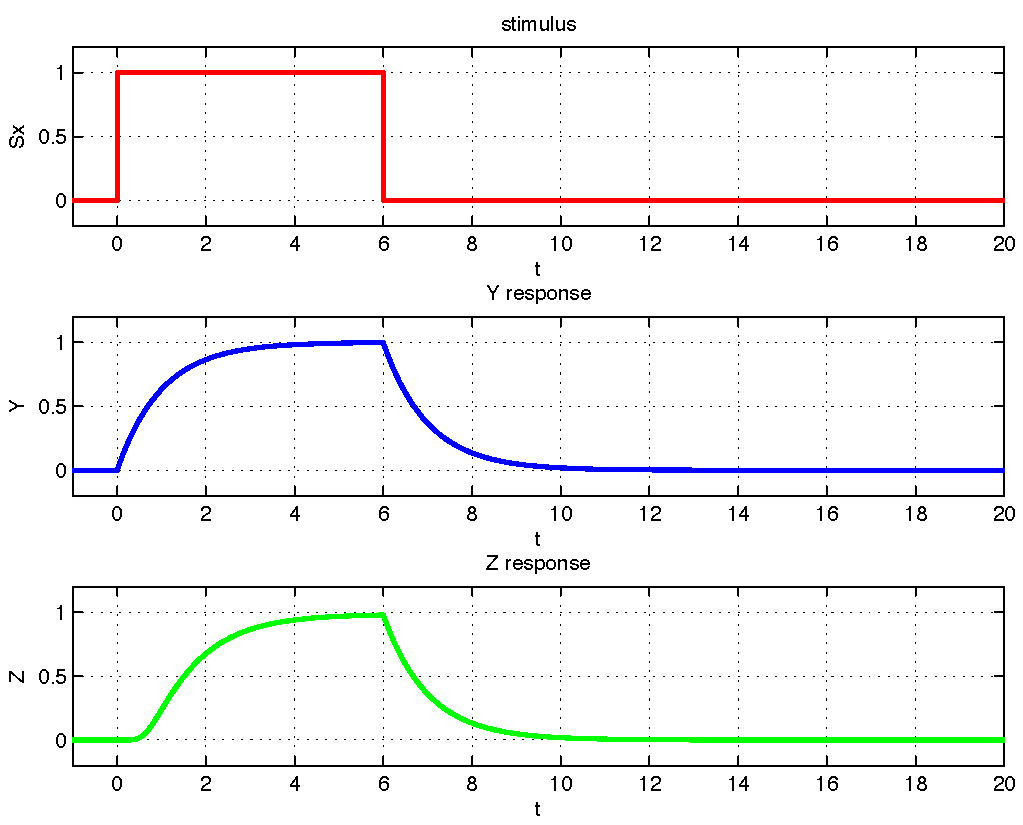
\includegraphics[scale=0.6]{plot_1A_AND} 
    \caption{Graphs illustrating system responses to the stimulus}
	\label{fig:plot_1A_AND}
\end{figure}

We report a delay in Z response after addition of the input signal \emph{$S_X$}
of $1.5200$. After the removal of the signal the concentratin on Z decreasing
immediately (no delay reported).
\newpage
\section{b}


\begin{figure}[h!]
 \centering
    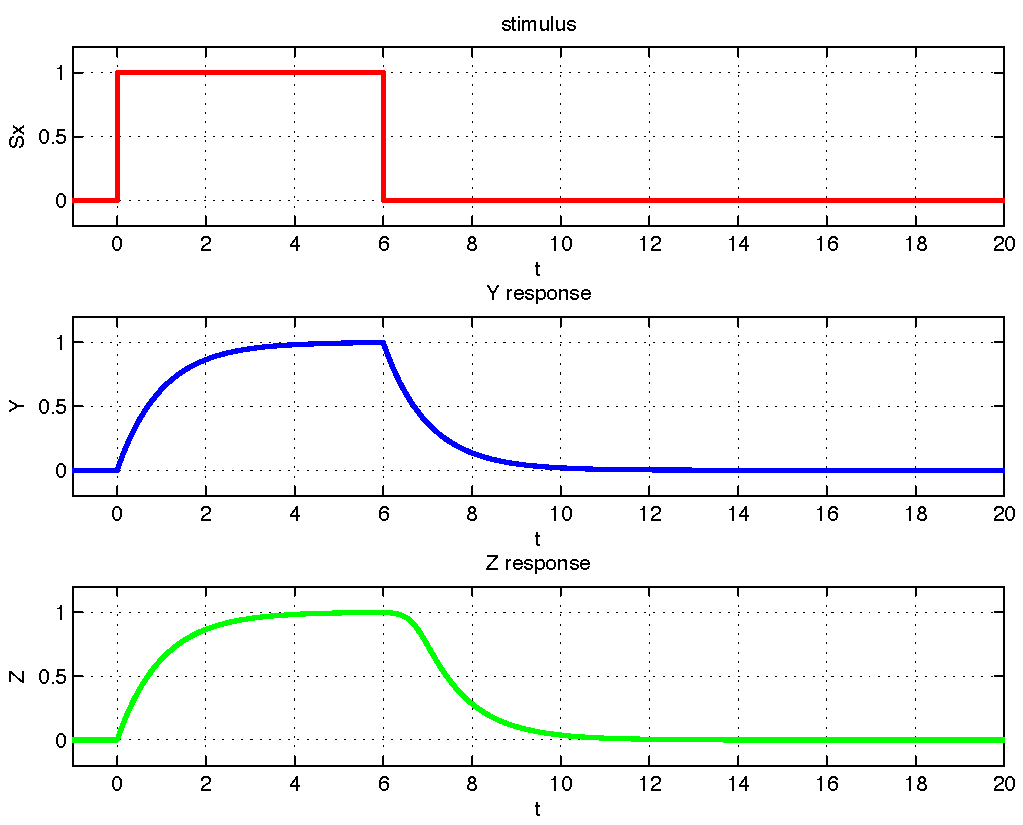
\includegraphics[scale=0.60]{plot_1B_OR} 
    \caption{Graphs illustrating system responses to the stimulus with OR
    gate and $K_{YZ} = 0.1 $}
	\label{fig:plot_1A_OR}
\end{figure}

\section{c}

\begin{table}[h!]
\begin{center}
\begin{tabular}{|l|rr|rr|r|}
\hline
Condition & Begin & End & Time begin & Time end & Duration \\
\hline
STD & $x>0$ & $x=0$ & $0.20$ & $15.88$ & $15.60$\\ 
\hline
\bottomrule
\end{tabular}
\caption{Computation of the maximum duration of the signal (STD)}
\end{center}
\end{table}			

\newpage
\section{d}

\begin{figure}[h!]
 \centering
    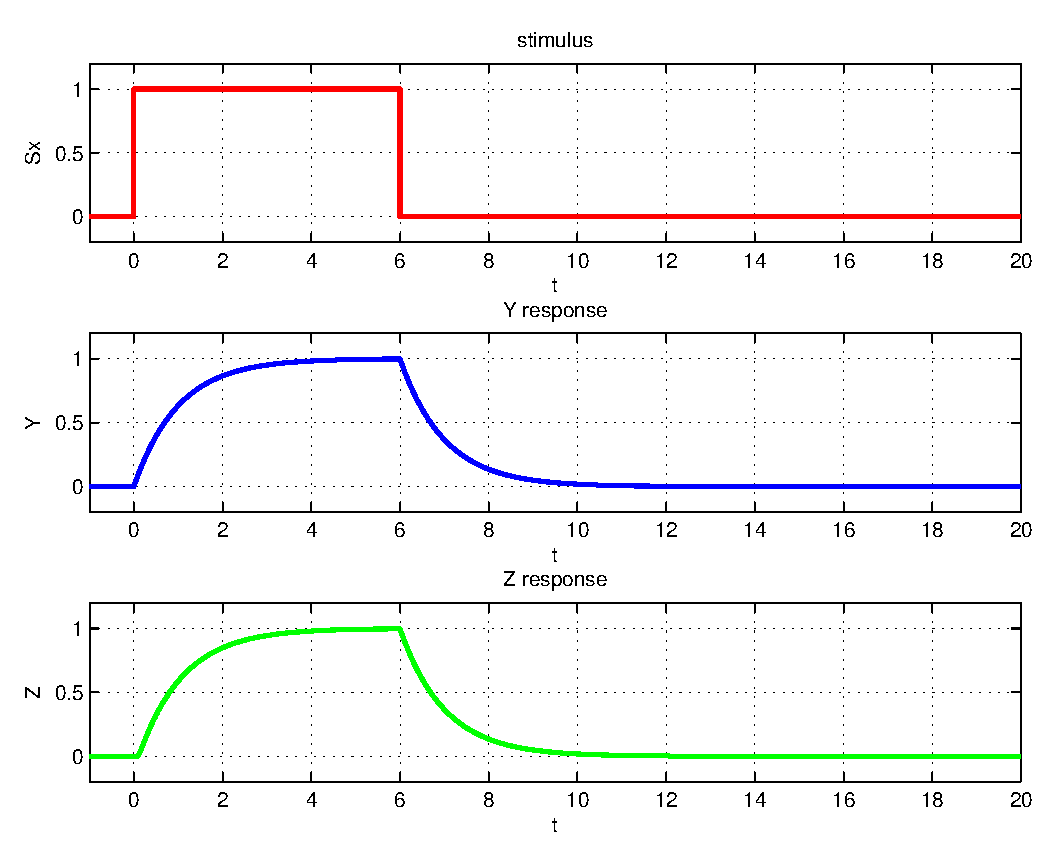
\includegraphics[scale=0.60]{plot_1D_01} 
    \caption{Graphs illustrating system responses to the stimulus with AND
    gate and $K_{YZ} = 0.1 $}
	\label{fig:plot_1D_01}
\end{figure}

\begin{figure}[h!]
 \centering
    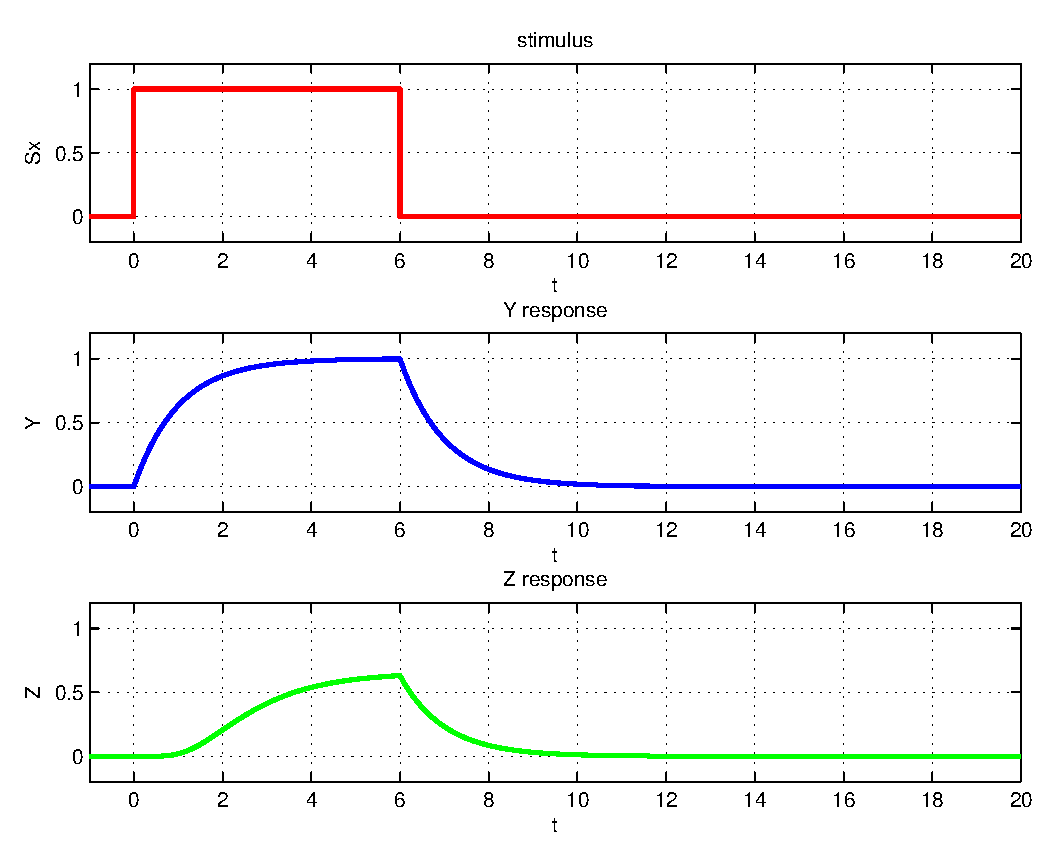
\includegraphics[scale=0.60]{plot_1D_09} 
    \caption{Graphs illustrating system responses to the stimulus with AND
    gate and $K_{YZ} = 0.9 $}
	\label{fig:plot_1D_09}
\end{figure}

\begin{table}[h!]
\begin{center}
\begin{tabular}{|l|rr|rr|r|}
\hline
Condition & Begin & End & Time begin & Time end & Duration \\
\hline
$K_{YZ} = 0.1$ & $x>0$ & $x=0$ & $0.05$ & $15.90$ & $15.85$\\ 
$K_{YZ} = 0.9$ & $x>0$ & $x=0$ & $0.34$ & $15.44$ & $15.10$\\ 
\hline
\bottomrule
\end{tabular}
\caption{Computation of the maximum duration of the signal ($K_{YZ} = 0.1$ and
$K_{YZ} = 0.9$)}
\end{center}
\end{table}	


\newpage

\setcounter{chapter}{4}
\setcounter{section}{0}

% \begin{section}{callODE.m}
% \lstinputlisting[caption={./callODE.m},label=lst:callODE-full]{./matlab_code/callODE.m}
% \end{section}
% \begin{section}{toggle.m}
% \lstinputlisting[caption={./toggle.m},label=lst:toggle-full]{./matlab_code/toggle.m}
% \end{section}
% \begin{section}{conv.m}
% \lstinputlisting[caption={./conv.m},label=lst:conv-full]{./matlab_code/conv.m}
% \end{section}
% \begin{section}{propensities.m}
% \lstinputlisting[caption={./propensities.m},label=lst:propensities-full]{./matlab_code/propensities.m}
% \end{section}
% \begin{section}{ssa.m}
% \lstinputlisting[caption={./ssa.m},label=lst:ssa-full]{./matlab_code/ssa.m}
% \end{section}


\bibliographystyle{plainnat}
\bibliography{science}

\backmatter


\end{document}